% Voir objectif SMART https://fr.wikipedia.org/wiki/Objectifs_et_indicateurs_SMART
\begin{figure}
    \centering % Les figures doivent être centrées
    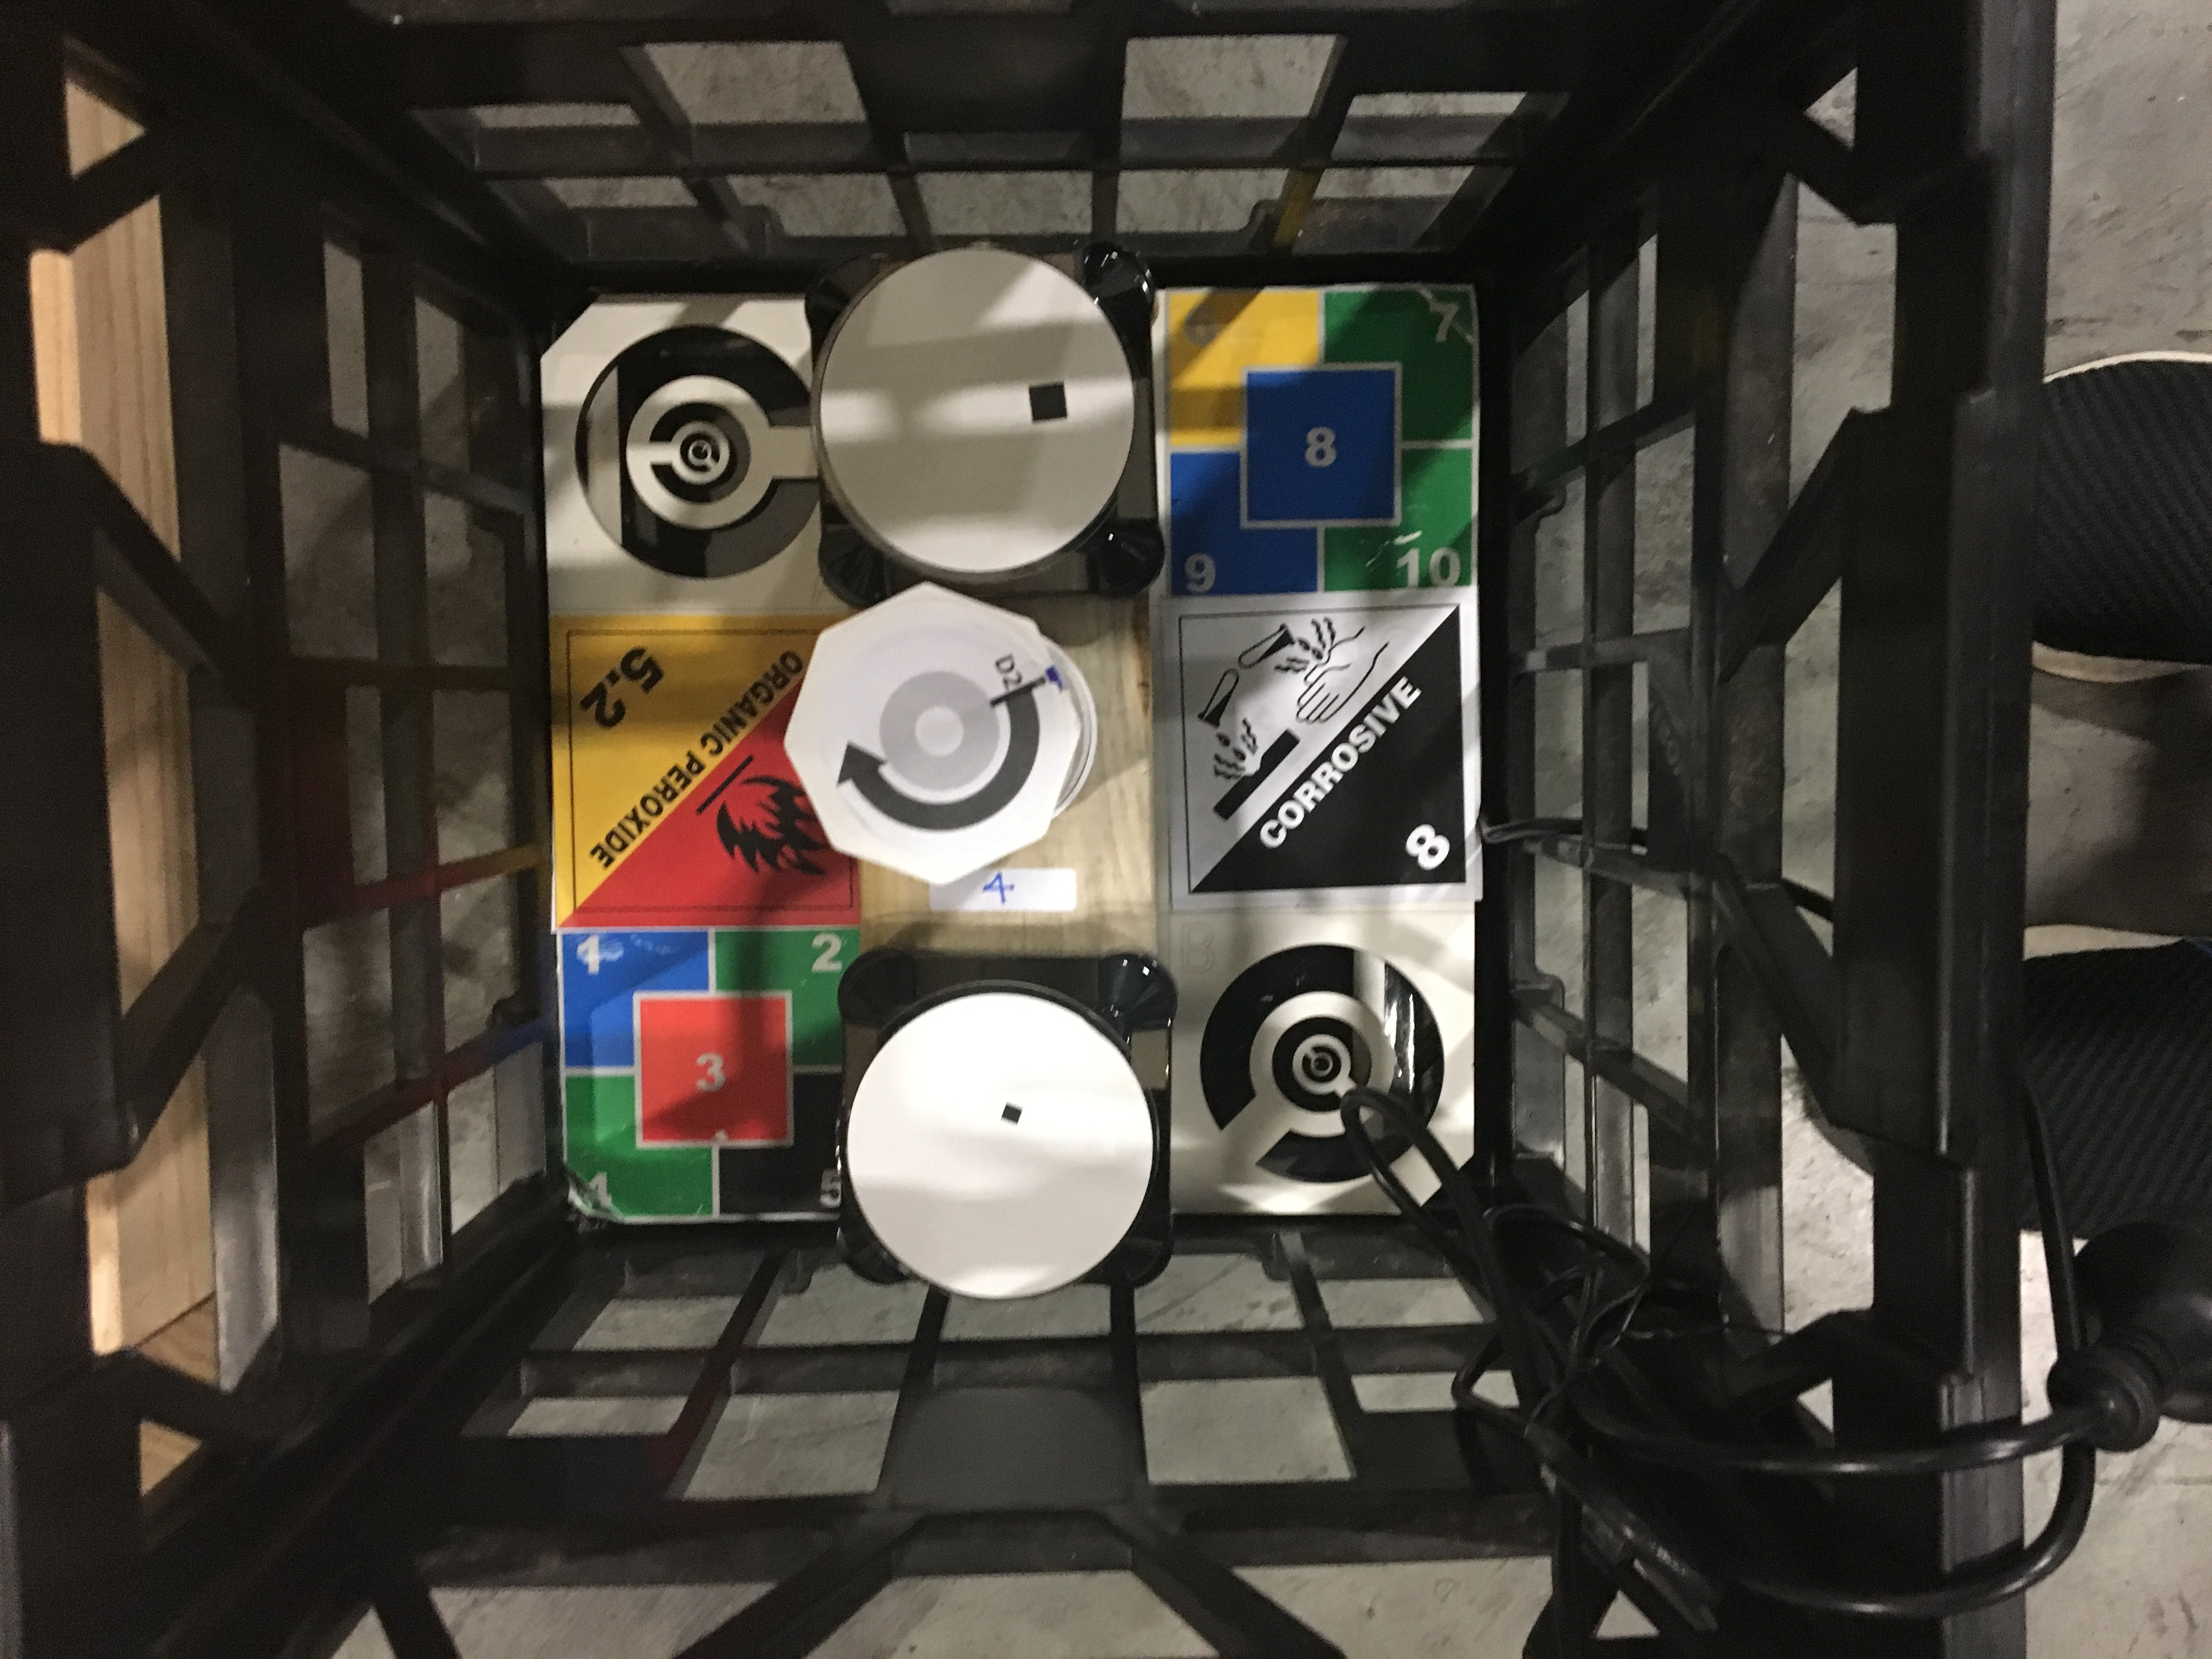
\includegraphics[width=0.75\textwidth]{Figures/test_method_rrl.JPG}
    \caption{Méthode d'essais de la RoboCup Rescue}
    \label{fig:test_method_rrl}
\end{figure}

L'objectif est de contrôler le bras robotique à l'aide d'instructions de mouvement cartésien. 
Le bras devra tenir compte de l'environnement qui l'entoure afin d'éviter une collision. La méthode d'essais qui sera utilisé à la RoboCup Rescue consiste à faire pivoter un tube de plastique PVC de 180 degrés puis de le retirer dans l'axe d'un autre tube de plus gros diamètre, le tuyau doit ensuite être déposé dans la caisse de lait. La figure \ref{fig:test_method_rrl} montre le banc d'essais qui met à l'épreuve les robots sur leur capacité à interagir avec les éléments de leur environnement. 
En ajout à l'objectif principal, on définira l'objectif plus ambitieux de contrôler le bras robotique à l'aide d'une souris 3D. La pince devra aussi être contrôlable en position, la vitesse d'ouverture/fermeture ainsi que la force de préhension seront contrôlables par les paramètres de l'interface utilisateur (UI) pour le moment.

